\chapter{可解释性分析}
\label{chap:5}

\section{基于SHAP的归因分析}
为了对深度神经网络在野火预测任务中的特性进行可解释性分析，本研究引入了基于博弈论理论的 SHAP（SHapley Additive exPlanations）解释框架。SHAP 的核心逻辑在于将模型对起火概率的预测视为一场由多种时空特征共同参与的“合作博弈” 。通过计算每个特征在所有可能的特征组合中带来的边际贡献，SHAP 能够为每一个输入变量分配一个量化的贡献值，即 SHAP 值。  
在数学表达上，SHAP 属于加性特征归因方法。对于一个特定的输入样本，其模型预测输出 $f(x)$ 可以表示为基线值（全体样本预测均值）与各个特征贡献值的线性累加：
\begin{equation}
     f(x) = \phi_0 + \sum_{i=1}^{M} \phi_i 
\end{equation}
其中，$\phi_0$ 为模型在无特征输入时的基础期望，$\phi_i$ 为第 $i$ 个特征的 SHAP 值。对于单个特征 $i$ 的 Shapley 值 $\phi_i$，其严格的理论计算公式如下：
\begin{equation}
    \phi_i = \sum_{S \subseteq F \setminus \{i\}} \frac{|S|!(|F| - |S| - 1)!}{|F|!} [f_{S \cup \{i\}}(x_{S \cup \{i\}}) - f_S(x_S)] 
\end{equation}

此处，$F$ 代表全体特征集合，$S$ 是不包含特征 $i$ 的任一特征子集。该公式通过对所有可能的特征排列顺序进行加权平均，确保了归因结果具备局部准确性、缺失性和一致性等优良数学性质。
SHAP（SHapley Additive exPlanations）是一种基于博弈论（Game Theory）中 Shapley 值的机器学习模型解释方法。其核心思想是将模型在特定样本上的预测结果视为各个输入特征（如气象、地貌、植被等）共同参与的一场“合作博弈”。模型最终的预测值与全体样本平均预测值（基线值）之间的偏差，被公平地分配给每个输入特征，这个分配值即为该特征的 SHAP 值。

在深度学习任务中，考虑到本研究所采用的 DualBranchSwinGCA 模型集成了 3D 滑动窗口注意力机制与地理感知交叉注意力（Geo-CA）模块，其内部梯度路径具有高度的非线性与复杂性。DeepSHAP 方法在处理此类自定义算子时容易出现算子不支持或梯度断裂的问题。因此，本实验采用了更为稳健的 GradientExplainer 解释器。该方法基于预期梯度（Expected Gradients）理论，通过在背景样本（Background Samples）和待解释样本之间进行路径积分，能够更稳健地分解模型在时空多模态输入下的预测逻辑。

在具体实施过程中，本研究首先筛选了 20 个未着火的负样本构建背景基线，用以代表环境的期望。由于模型输入包含地理坐标等非计算类元数据，本实验设计了一个模型包装器（Wrapper），将不参与特征提取的变量进行屏蔽，从而确保 SHAP 解释器能够聚焦于真正驱动火灾蔓延的特征变量。针对待解释的火灾正样本，本实验选取了 30 个具有代表性的真实火灾样本进行分批归因计算，通过在输入空间与背景空间之间进行路径梯度积分，计算出各要素的边际贡献,并取其 SHAP 绝对值的均值 $mean(\|SHAP\|)$ 作为衡量特征全局重要性的核心指标。为了清晰地展示不同维度特征的贡献，我们将输入特征划分为动态气象特征、静态地理特征以及地表覆盖类型特征（CLC），得到的全局变量贡献度排序如图 \ref{fig:5-1-shap} 所示。

\begin{figure}[htbp]
    \centering
    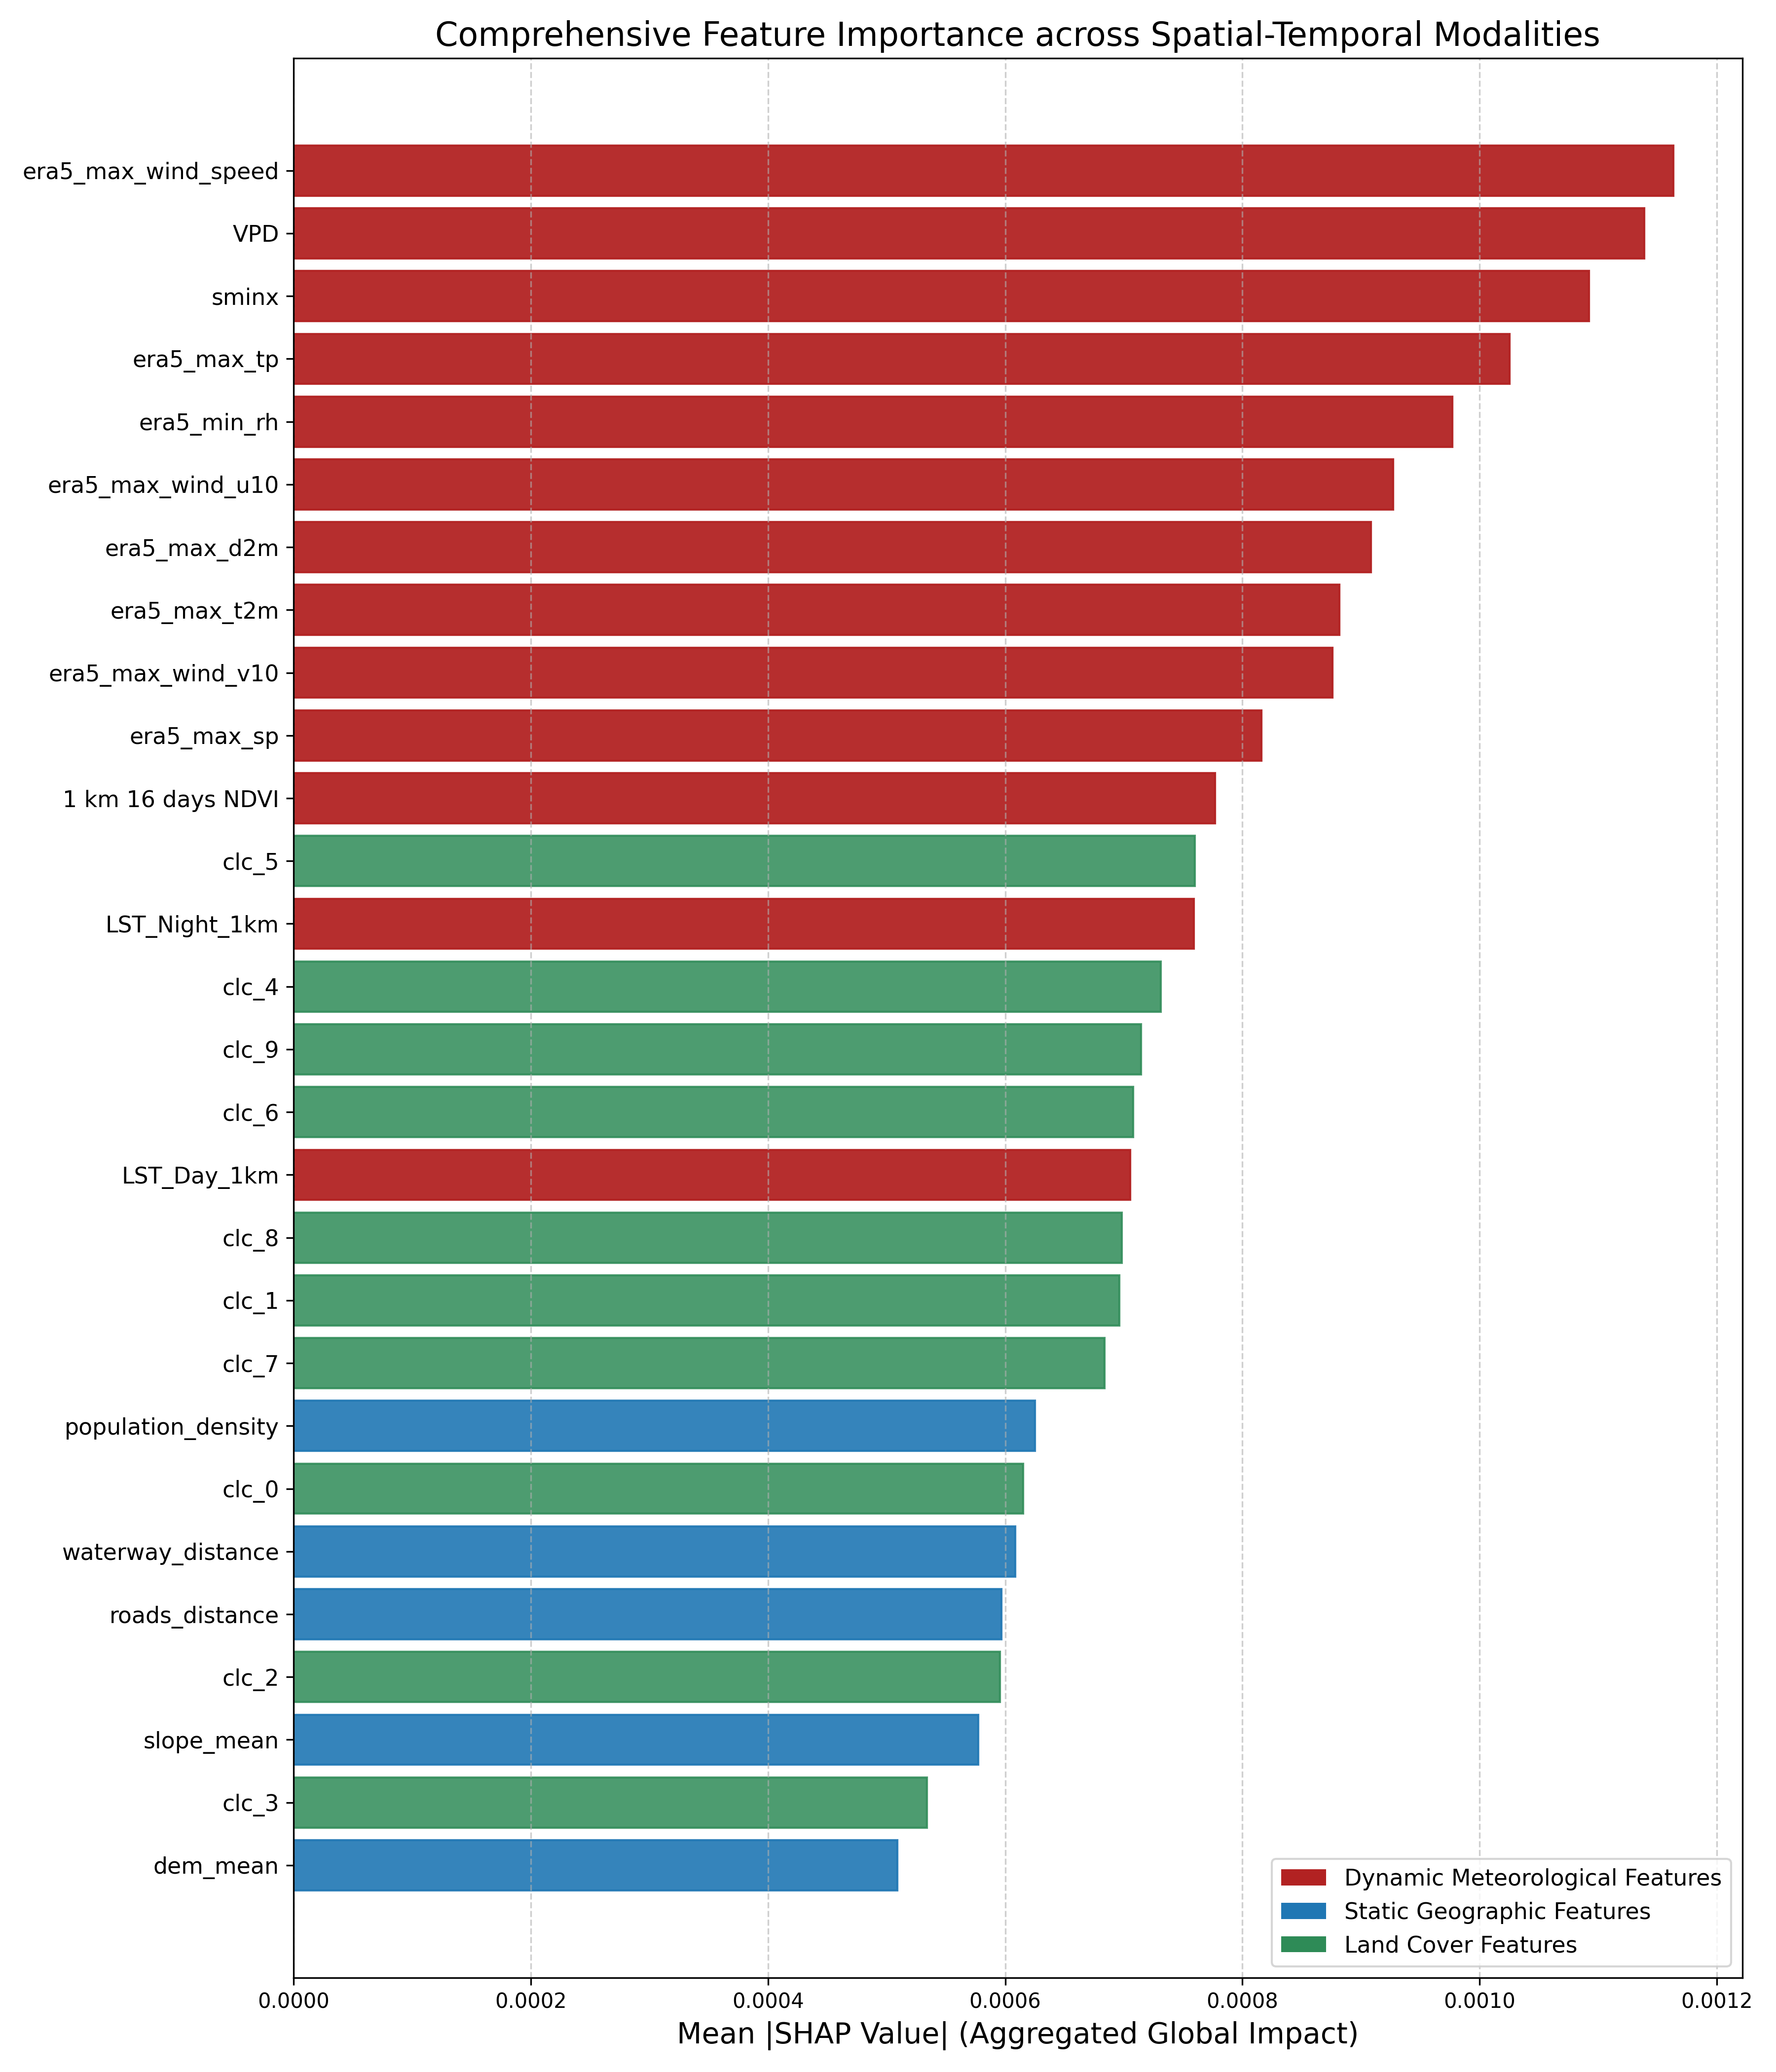
\includegraphics[width=0.9\textwidth]{img/chap5/5-1-shap-all.png}
    \caption{特征变量的SHAP值排序}
    \label{fig:5-1-shap}
\end{figure}

实验结果表明，动态气象特征在模型预测过程中起主导作用。其中，最大风速（$era5_max_wind_speed$）的特征重要性最高，而风场的两个分量 $wind_u10$ 与 $wind_v10$ 同样具有较高贡献。这说明风场信息对野火蔓延方向与传播速度具有显著影响，也从侧面验证了本文引入风场动力学偏置机制的合理性。此外，本文构建的饱和水汽压差（VPD）特征也表现出较高的重要性，其贡献高于传统的相对湿度与气温变量。这表明，相较于单一气象指标，VPD 能够更有效地反映空气干燥程度，以及可燃物失水状态，从而帮助模型更准确地识别高火险环境。

与动态特征相比，静态地理特征如海拔（$dem\_mean$）和坡度（$slope\_mean$）对预测结果的贡献相对较小。在土地覆盖特征方面，不同类别的植被类型展现了差异化的贡献度。总体上牧场和普通农用地的SHAP特征值较大，模型在计算时赋予了这些区域更高的权重。

\section{对于特征融合模块Geo-CA的空间交叉注意力分析}
本小节旨在探究地理感知交叉注意力（Geo-CA）模块是否能对动态变量和静态变量双分支进行融合，并基于风向矢量这一动力学特征进行偏置。故本节针对较大风速条件下的火灾样本，进行了空间注意力的提取与可视化分析。

具体提取与可视化方法如下，选取待预测的中心目标网格作为注意力计算的 Query，将周围的广阔空间上下文作为 Keys。通过截获模型前向传播过程中的 $saved_attn_weights$，提取出该中心网格对周围所有区域的注意力分配权重矩阵。由于经过网络的多层下采样，提取出的注意力图尺度为 $7\times 7$。为了与真实的物理空间对齐并便于可视化，本研究采用双三次插值（Bicubic Interpolation）算法，将其平滑上采样还原至原始的$25\times 25$空间分辨率，并进行 Min-Max 归一化处理。

\begin{figure}[htbp]
    \centering
    \begin{minipage}{0.45\textwidth}
        \centering
        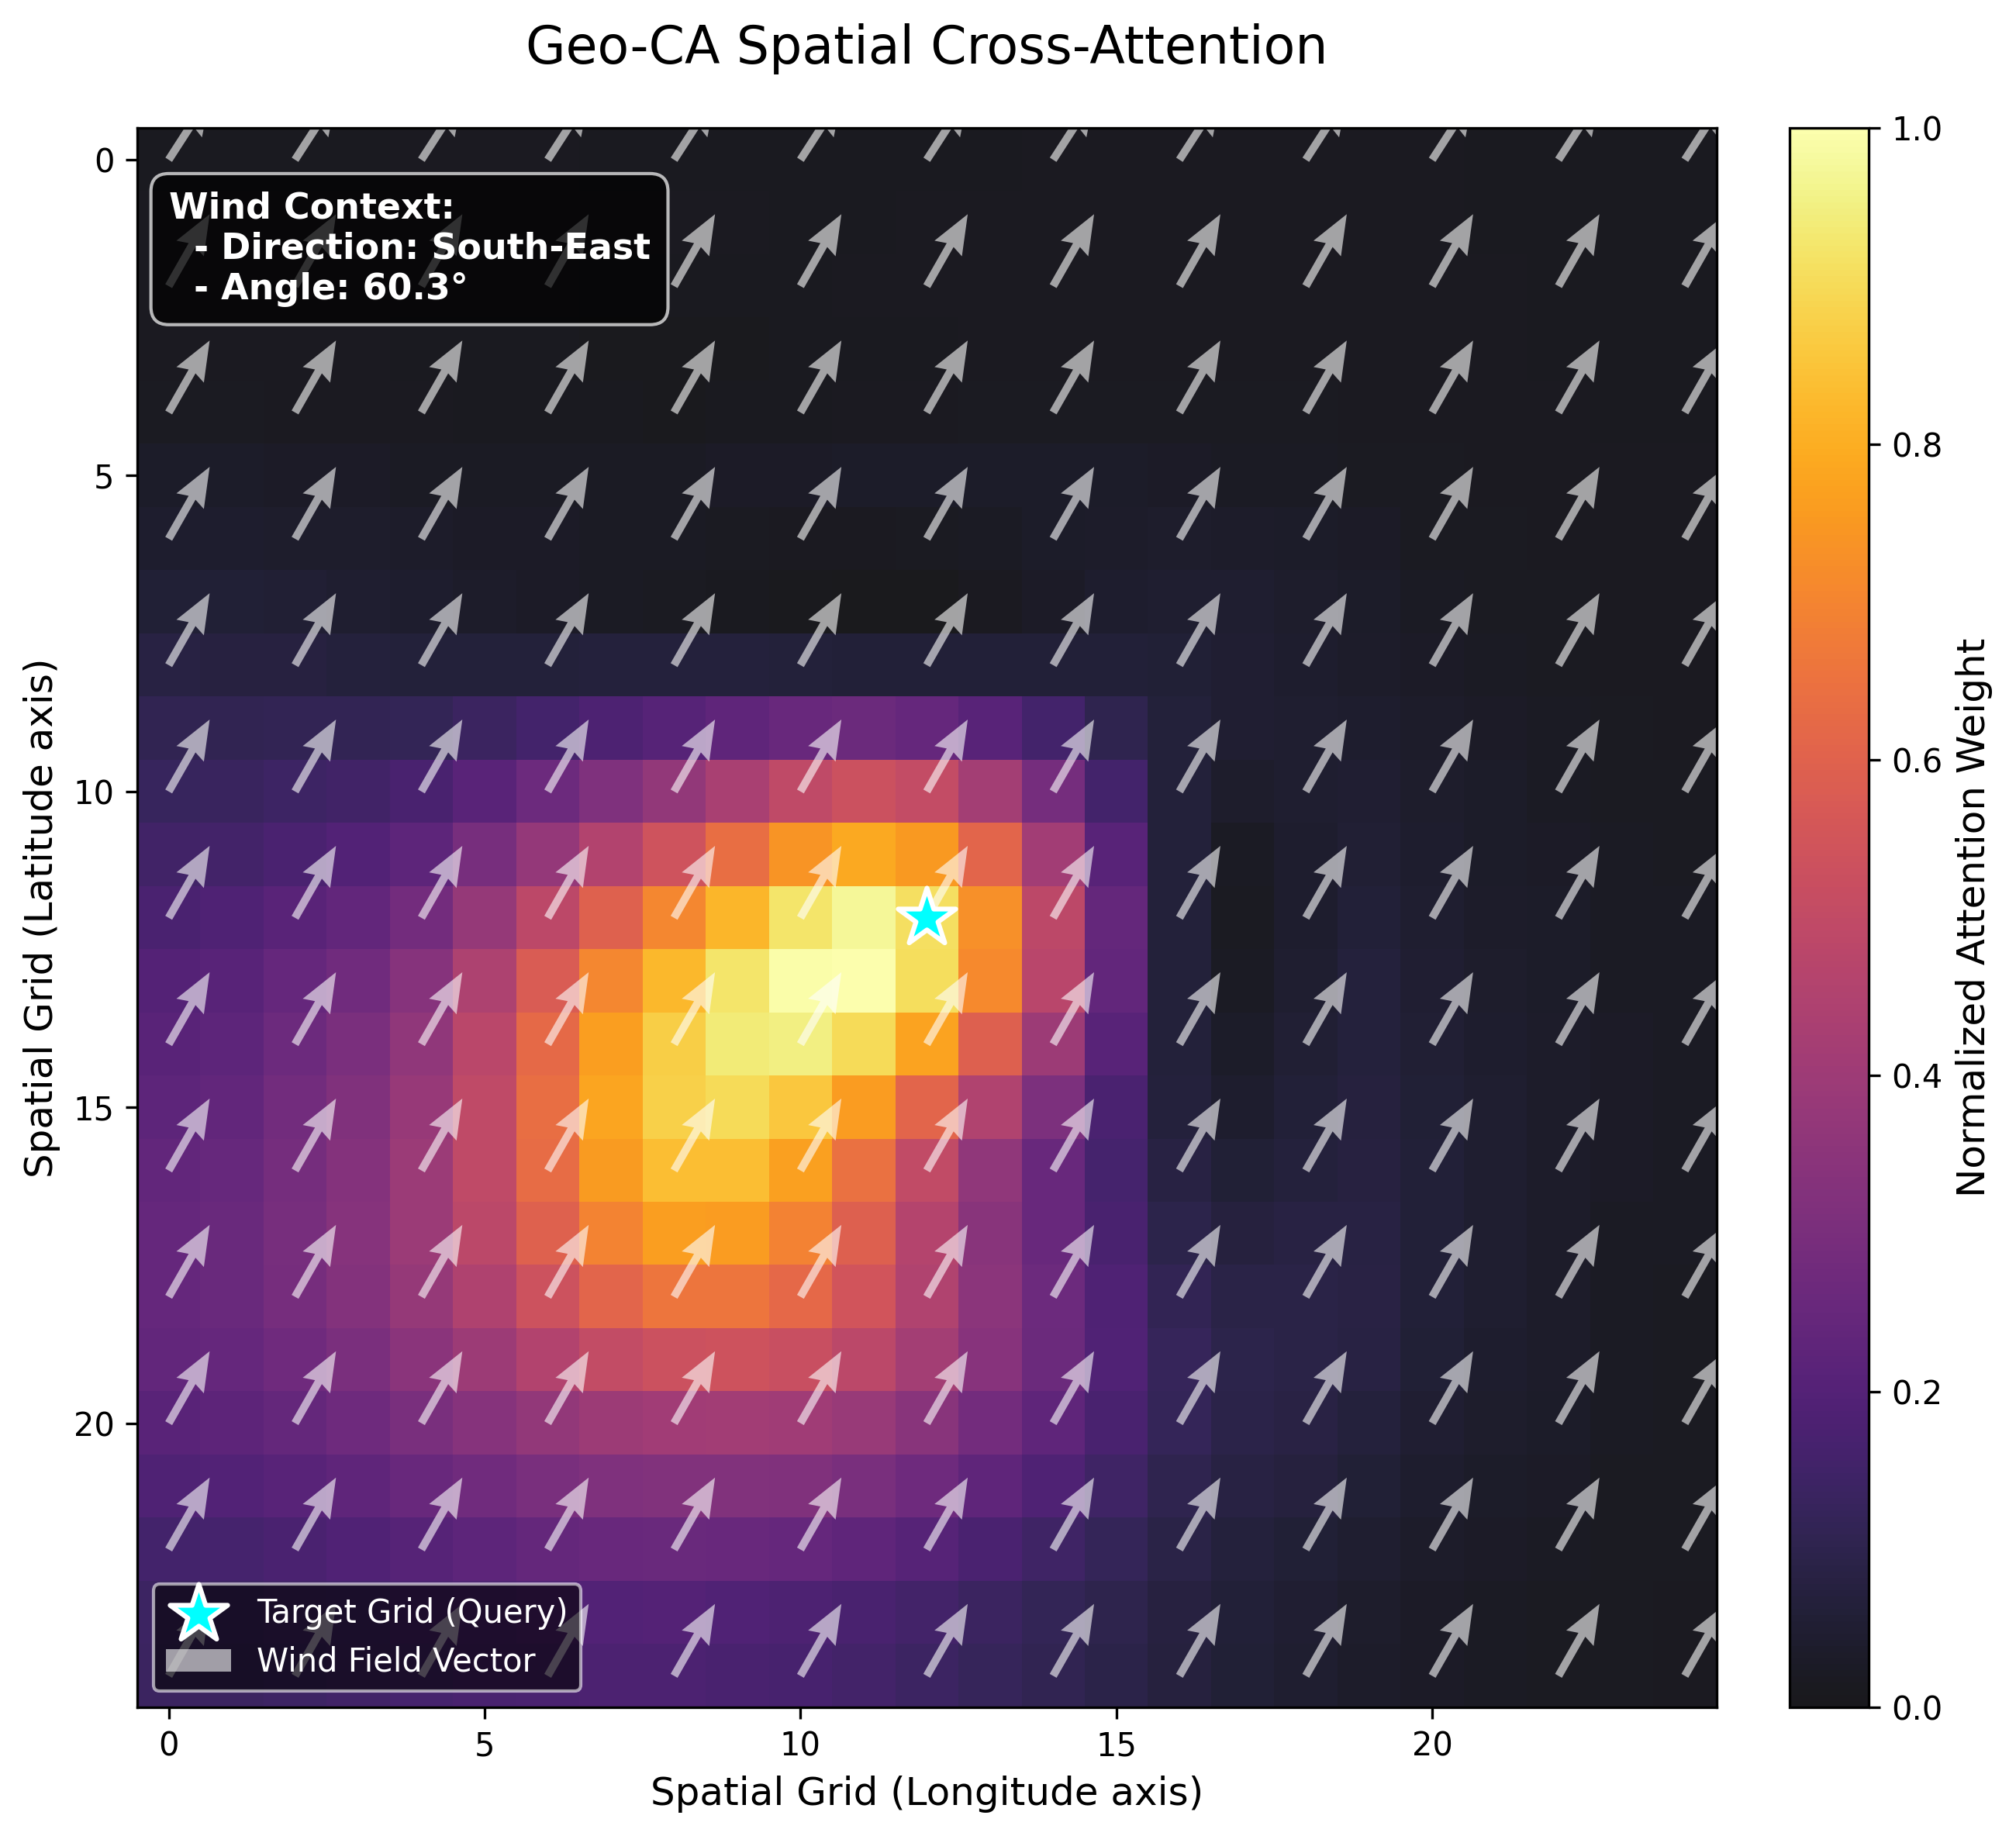
\includegraphics[width=\linewidth]{img/chap5/5-2-wind-attention-1.png} 
        \centerline{(a) 西南风，风速较大}
    \end{minipage}\hfill
    \begin{minipage}{0.45\textwidth}
        \centering
        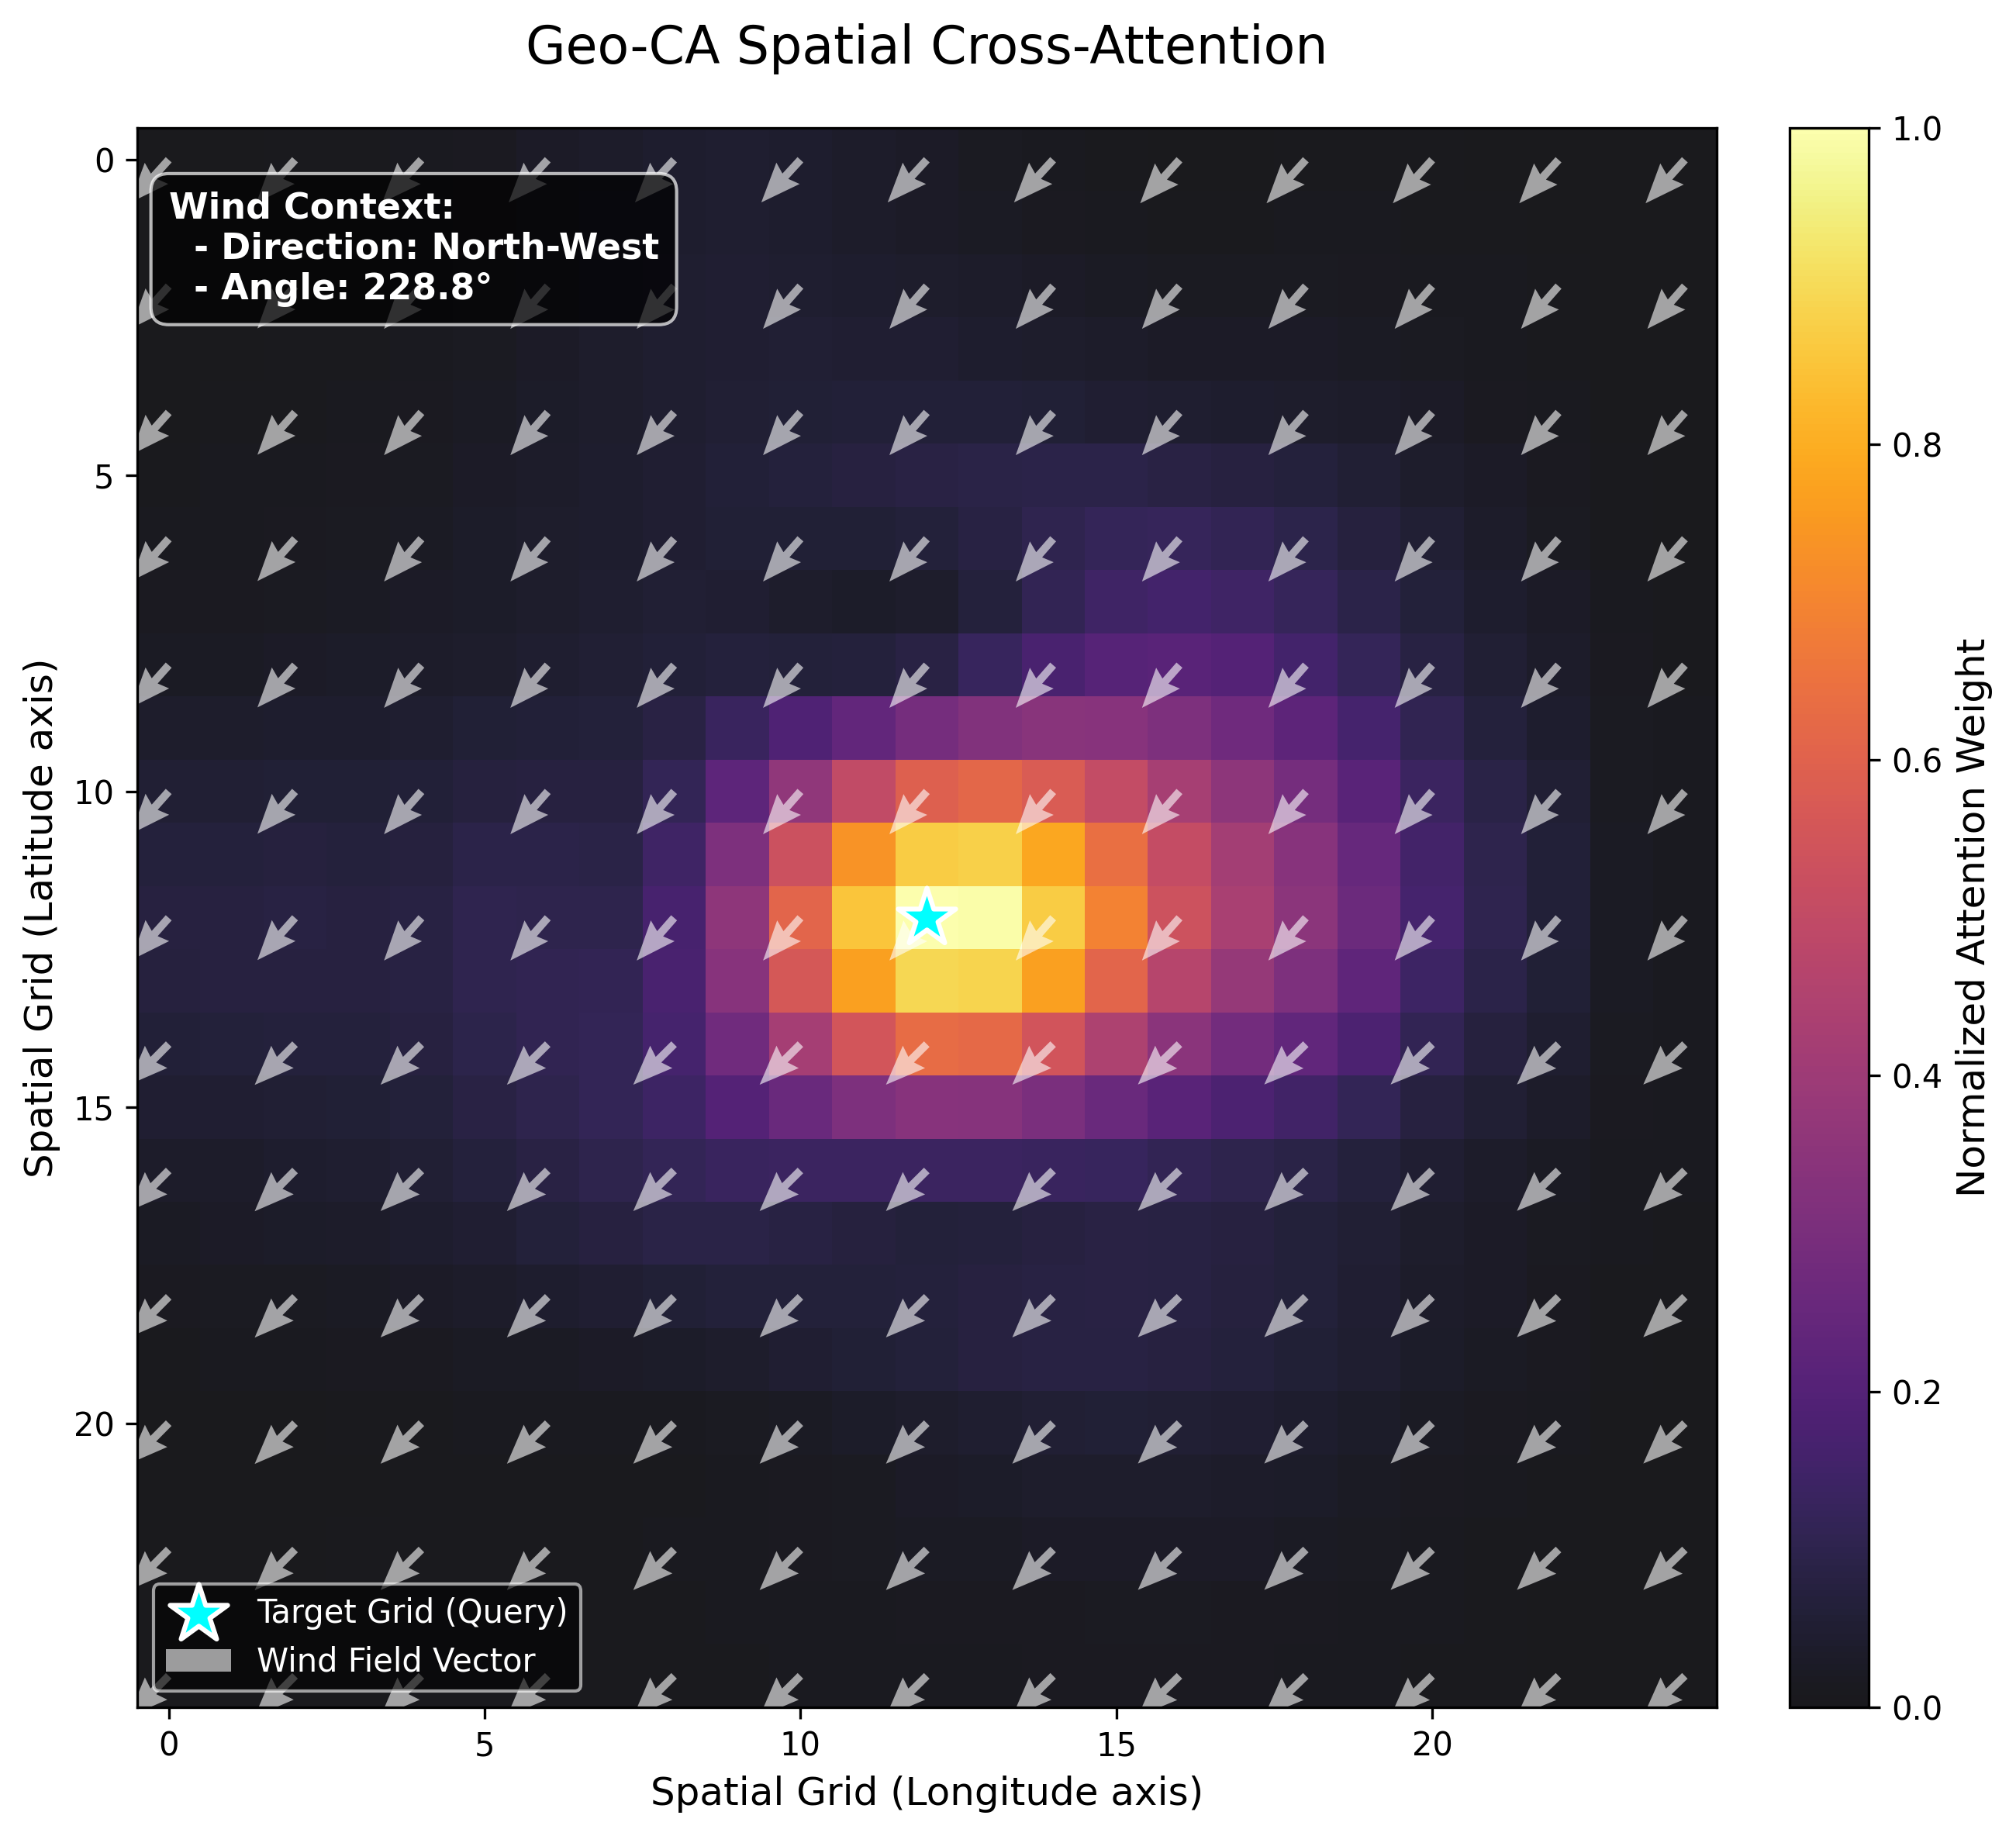
\includegraphics[width=\linewidth]{img/chap5/5-2-wind-attention-2.png} 
        \centerline{(b) 东北风，风速较小}
    \end{minipage}
    \caption{风场矢量对Geo-CA的空间注意力权重的影响}
    \label{fig:5-2-wind-attention}
\end{figure}

图\ref{fig:5-2-wind-attention}展示了风场矢量对Geo-CA的空间注意力权重的影响。图中箭头代表风场矢量，即箭头的方向代表风速的方向，箭头的长短代表风速的大小。对比(a)(b)两图可以看出，图(a)处于高风速环境，而图(b)处于低风速环境。对比两者的底层热力图可以发现：在风速较大的图(a)中，模型的高亮注意力区域明显向外扩散，呈现出更大的空间感受野；而在风速较小的图(b)中，注意力权重则较收敛、集中在预测中心点附近。此外，风向也影响了注意力权重的空间偏移。如对比图所示，注意力高度集中的高亮区域并非随机分布，而是与风向矢量的轴线存在显著的重合。更为关键的是，模型赋予了风的来向（即上风向区域）更大的注意力权重。

上述分析证明了风向矢量融入Geo-CA模块的有效性，Geo-CA 模块并非单纯的数学注意力映射，而能够根据风场矢量等物理特征进行注意力的偏置，从而为野火蔓延的预测注入物理学信息。

类似地，提取模型在 Geo-CA 融合前后的特征激活图（Feature Activation Maps）并进行可视化对比，图\ref{fig:5-2-branch-attention}分别展现了模型的静态特征激活图、动态特征激活图及融合后的最终激活状态的一个例子。观察可知，融合后的注意力区域并非左图与中图的简单线性叠加，而是同时捕获了静态与动态特征图的关键特征，证明了Geo-CA融合机制的有效性，也证明了双分支Swin Transformer结构的高效性。
\begin{figure}[htbp]
    \centering
    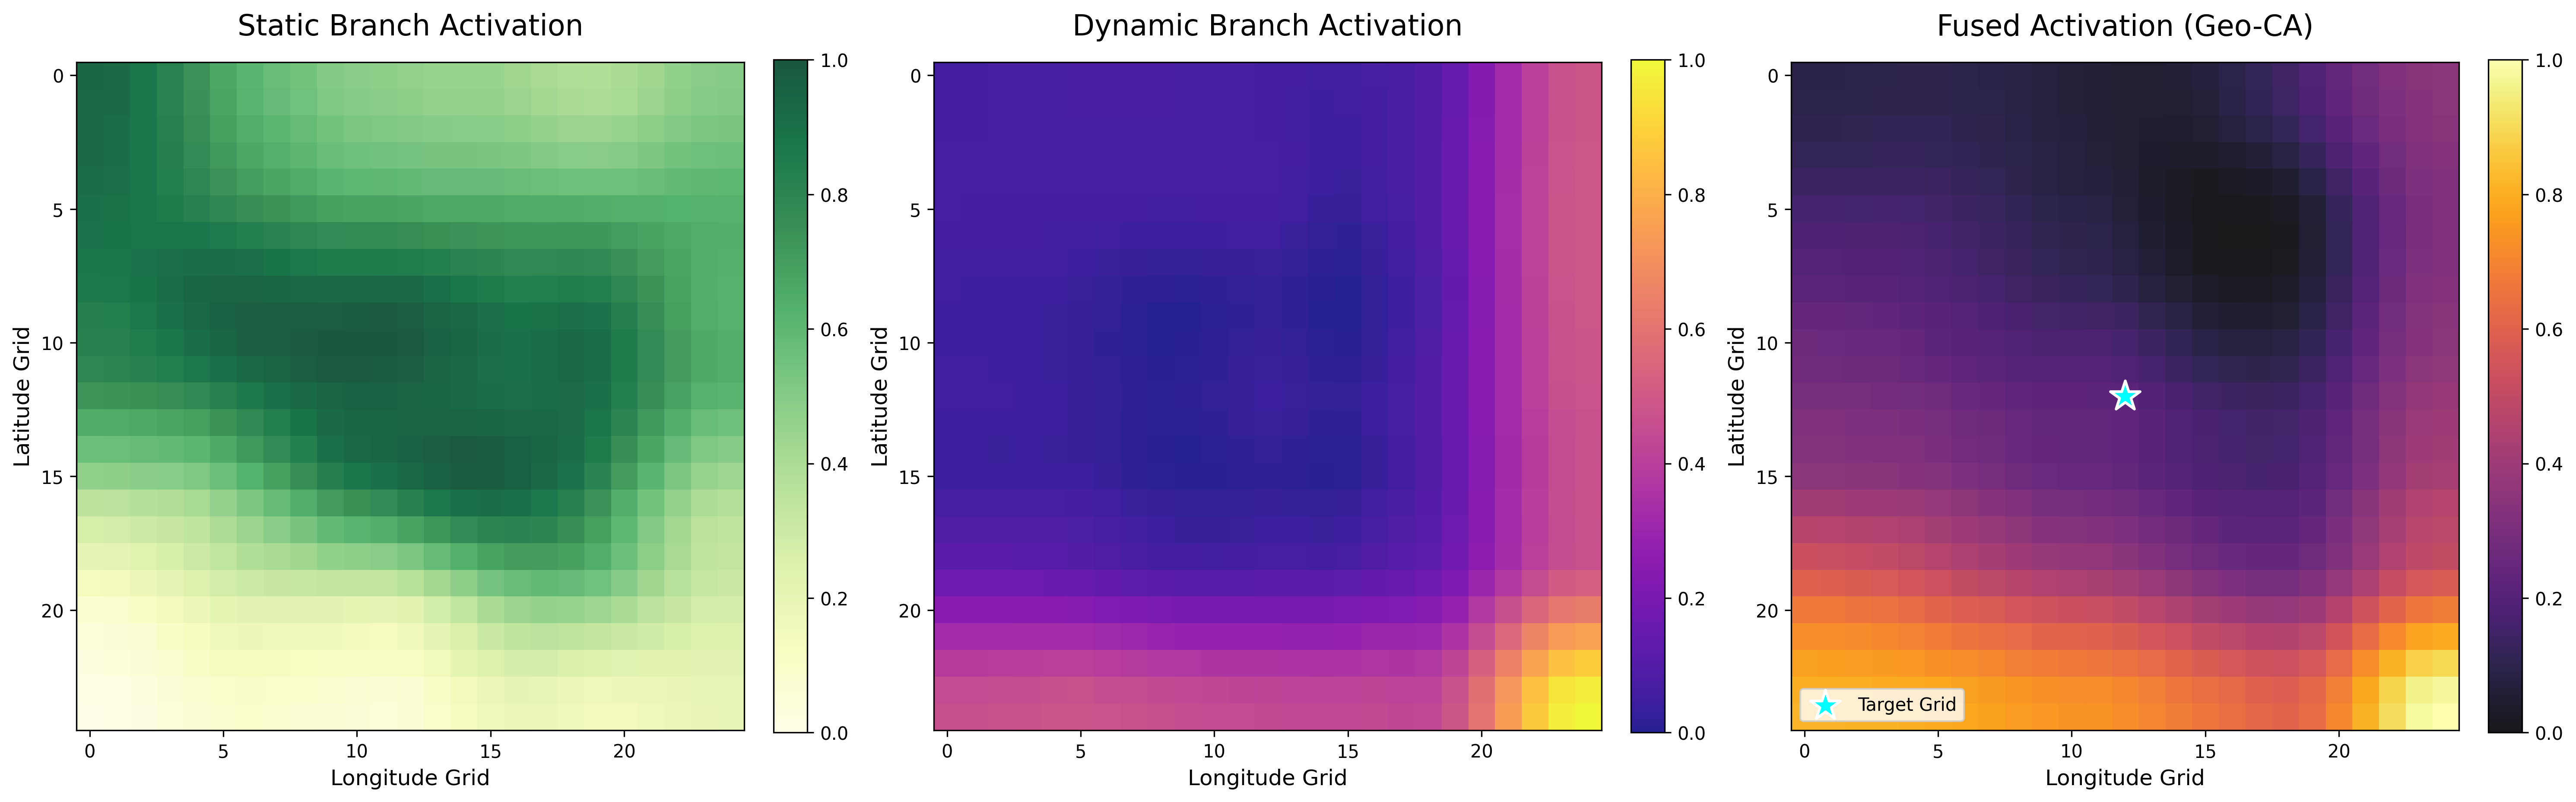
\includegraphics[width=0.9\textwidth]{img/chap5/5-2-branch-attention-1.png}
    \caption{Geo-CA 融合前后的特征激活图}
    \label{fig:5-2-branch-attention}
\end{figure}

本章针对深度学习模型的内部机制，进行了对本研究模型的可解释性分析。首先，利用基于博弈论的 SHAP 方法，探究了不同特征变量对野火预测的贡献程度。归因结果表明，最大风速和本研究引入的饱和水汽压差（VPD）等动态变量在野火预测中起到了主导作用，且不同土地覆盖类型呈现出差异化贡献，证明模型准确学习到了野火演化的核心动力学与热力学机制。其次，针对地理感知交叉注意力（Geo-CA）模块进行了可视化探究。通过对比不同风速与风向条件下的注意力分布，发现其能够打破各向同性的空间注意力计算限制，对风向矢量偏置做出注意力响应。特征激活图对比则展现了双分支结构的解耦提取能力，以及 Geo-CA 作为融合机制的精准有效。综合上述分析，验证了本研究提出的模型架构具备科学合理性与物理可解释性。